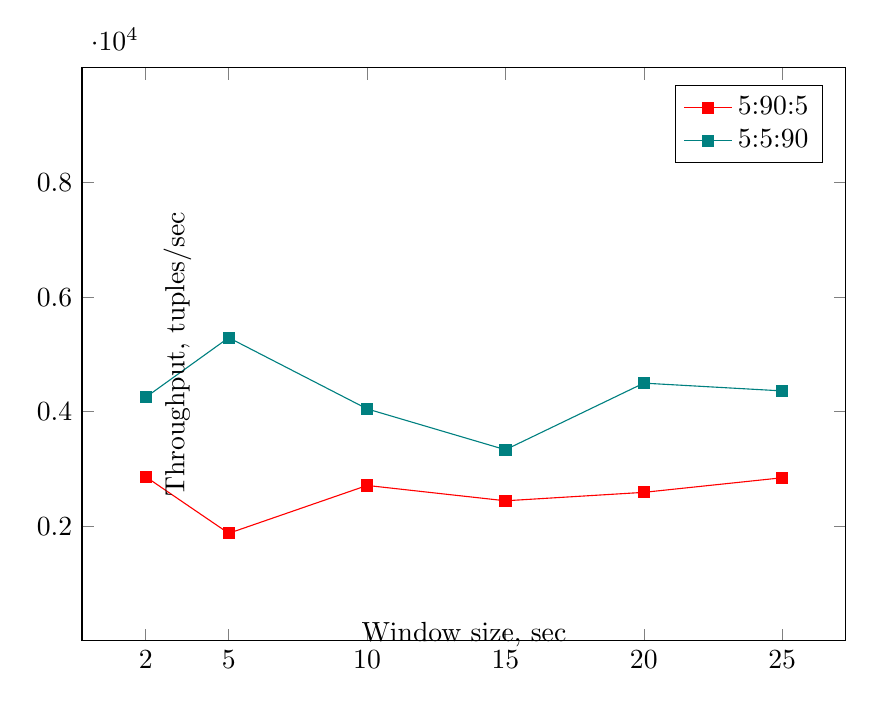
\begin{tikzpicture}
\begin{axis}[
    scale only axis=true,
    width=0.8\textwidth,
    height=0.6\textwidth,
    ymin = 0,
    ymax = 10000,
    ytick={2000, 4000, 6000, 8000},
    %yticklabels={2, 4, 6, 8},
    xtick={2, 5, 10, 15, 20, 25},
    xticklabels={$2$, $5$, $10$, $15$, $20$, $25$},
    legend cell align=left,
    legend pos=north east,
    xlabel={Window size, sec},
    ylabel={Throughput, tuples/sec},
    x label style={at={(axis description cs:0.5,0.05)},anchor=north},
    y label style={at={(axis description cs:0.125,0.5)},anchor=center},
]
\addplot[red, mark=square*, mark options={scale=1,solid}] coordinates {
(2,2863.74)
(5,1876.12)
(10,2711.66)
(15,2443.98)
(20,2591.34)
(25,2845.98)
};
\addplot[teal, mark=square*, mark options={scale=1,solid}] coordinates {
(2,4250.0)
(5,5291.2)
(10,4048.2)
(15,3335.0)
(20,4497.8)
(25,4362.1)
};
\legend{
    5:90:5\\
    5:5:90\\
}
\end{axis}
\end{tikzpicture}